%%%%%%%%%%%%%%%%%%%%%%%%%%%%%%%%%%%%%%%%%%%%%%%%%%%%%%%%%%%
%%%%%%%%%%%%%%%%%%%%%%%%%%%%%%%%%%%%%%%%%%%%%%%%%%%%%%%%%%%
%%%%%%%%%%%%%%%%%%%%%%%%%%%%%%%%%%%%%%%%%%%%%%%%%%%%%%%%%%%

%% PREAMBLE! :-)


\documentclass[a4paper, 10pt]{article}

%%% packages - input should be path where your packages.tex file is saved.
%% packages

\usepackage{setspace}

%%%%%%%%%%%%%%%%%%%%%%%%%%%%%%%%%%%%%
%%%%%%%%%%%%%%%%%%%%%%%%%%%%%%%%%%%%%
%%%%%%%%%%%%%%%%%%%%%%%%%%%%%%%%%%%%%

%%% This is a package to use UTF8 CSV files as input and directly convert them to latex tables.
\usepackage{csvsimple}
%https://texblog.org/2012/05/30/generate-latex-tables-from-csv-files-excel/

%%%%%%%%%%%%%%%%%%%%%%%%%%%%%%%%%%%%%
%%%%%%%%%%%%%%%%%%%%%%%%%%%%%%%%%%%%%
%%%%%%%%%%%%%%%%%%%%%%%%%%%%%%%%%%%%%

\usepackage[version=4]{mhchem}
% package for using chemical equations and fonts 
% https://mirror.kumi.systems/ctan/macros/latex/contrib/mhchem/mhchem.pdf

%%%%%%%%%%%%%%%%%%%%%%%%%%%%%%%%%%%%%
%%%%%%%%%%%%%%%%%%%%%%%%%%%%%%%%%%%%%
%%%%%%%%%%%%%%%%%%%%%%%%%%%%%%%%%%%%%

\usepackage{xparse}
% high level user interface package, use with caution
% https://mirror.easyname.at/ctan/macros/latex/contrib/l3packages/xparse.pdf

%%%%%%%%%%%%%%%%%%%%%%%%%%%%%%%%%%%%%
%%%%%%%%%%%%%%%%%%%%%%%%%%%%%%%%%%%%%
%%%%%%%%%%%%%%%%%%%%%%%%%%%%%%%%%%%%%

\usepackage{makeidx}
\usepackage{pdfpages}
\usepackage{lastpage}

%%%%%%%%%%%%%%%%%%%%%%%%%%%%%%%%%%%%%
%%%%%%%%%%%%%%%%%%%%%%%%%%%%%%%%%%%%%
%%%%%%%%%%%%%%%%%%%%%%%%%%%%%%%%%%%%%

%%% Package to control inclusion and exclusion of specific entry in the table of contents.
%%% https://mirror.foobar.to/CTAN/macros/latex/contrib/tocbibind/tocbibind.pdf
\usepackage[nottoc,notlot,notlof]{tocbibind}

%%%%%%%%%%%%%%%%%%%%%%%%%%%%%%%%%%%%%
%%%%%%%%%%%%%%%%%%%%%%%%%%%%%%%%%%%%%
%%%%%%%%%%%%%%%%%%%%%%%%%%%%%%%%%%%%%

\usepackage{bigstrut}
% needed for crazy table commands, its cool trust me!
% https://anorien.csc.warwick.ac.uk/mirrors/CTAN/macros/latex/contrib/multirow/multirow.pdf

%%%%%%%%%%%%%%%%%%%%%%%%%%%%%%%%%%%%%
%%%%%%%%%%%%%%%%%%%%%%%%%%%%%%%%%%%%%
%%%%%%%%%%%%%%%%%%%%%%%%%%%%%%%%%%%%%

\usepackage{graphicx} 								
% Required for the inclusion of images
% https://de.overleaf.com/learn/latex/Inserting_Images

%%%%%%%%%%%%%%%%%%%%%%%%%%%%%%%%%%%%%
%%%%%%%%%%%%%%%%%%%%%%%%%%%%%%%%%%%%%
%%%%%%%%%%%%%%%%%%%%%%%%%%%%%%%%%%%%%

\usepackage{amsmath} 								
% Required for some math elements 
% https://www.namsu.de/Extra/pakete/amsmath/Amsmath.html

%%%%%%%%%%%%%%%%%%%%%%%%%%%%%%%%%%%%%
%%%%%%%%%%%%%%%%%%%%%%%%%%%%%%%%%%%%%
%%%%%%%%%%%%%%%%%%%%%%%%%%%%%%%%%%%%%

\usepackage{amssymb}
% required for some more crazy math elements, checks mal ab!
% http://milde.users.sourceforge.net/LUCR/Math/mathpackages/amssymb-symbols.pdf

%%%%%%%%%%%%%%%%%%%%%%%%%%%%%%%%%%%%%
%%%%%%%%%%%%%%%%%%%%%%%%%%%%%%%%%%%%%
%%%%%%%%%%%%%%%%%%%%%%%%%%%%%%%%%%%%%

%\usepackage{kbordermatrix} 	
% some special matrix-commands						
% http://www.hss.caltech.edu/~kcb/TeX/kbordermatrix.sty
%%%%%%%%%%%%%%%%%%%%%%%%%%%%%%%%%%%%%
%%%%%%%%%%%%%%%%%%%%%%%%%%%%%%%%%%%%%
%%%%%%%%%%%%%%%%%%%%%%%%%%%%%%%%%%%%%

\usepackage{multicol}								
% multicolumn-commands stuffs
% https://de.overleaf.com/learn/latex/Multiple_columns

%%%%%%%%%%%%%%%%%%%%%%%%%%%%%%%%%%%%%
%%%%%%%%%%%%%%%%%%%%%%%%%%%%%%%%%%%%%
%%%%%%%%%%%%%%%%%%%%%%%%%%%%%%%%%%%%%

\usepackage{color}
\definecolor{dkgreen}{rgb}{0,0.6,0}
\definecolor{gray}{rgb}{0.5,0.5,0.5}
\definecolor{mauve}{rgb}{0.58,0,0.82}
\definecolor{darkblue}{rgb}{0.0,0.0,0.6}
\definecolor{cyan}{rgb}{0.0,0.6,0.6}

%%%%%%%%%%%%%%%%%%%%%%%%%%%%%%%%%%%%%
%%%%%%%%%%%%%%%%%%%%%%%%%%%%%%%%%%%%%
%%%%%%%%%%%%%%%%%%%%%%%%%%%%%%%%%%%%%

% package to more precisely wrap your document around ur figure!
% https://de.overleaf.com/learn/latex/wrapping_text_around_figures
\usepackage{wrapfig}								

%%%%%%%%%%%%%%%%%%%%%%%%%%%%%%%%%%%%%
%%%%%%%%%%%%%%%%%%%%%%%%%%%%%%%%%%%%%
%%%%%%%%%%%%%%%%%%%%%%%%%%%%%%%%%%%%%

% the package for bold math symbol commands!
% https://anorien.csc.warwick.ac.uk/mirrors/CTAN/macros/latex/required/tools/bm.pdf
\usepackage{bm}

%%%%%%%%%%%%%%%%%%%%%%%%%%%%%%%%%%%%%
%%%%%%%%%%%%%%%%%%%%%%%%%%%%%%%%%%%%%
%%%%%%%%%%%%%%%%%%%%%%%%%%%%%%%%%%%%%

% subcaption package dependant on caption package (self-explanatory)
% https://www.namsu.de/Extra/pakete/Subcaption.html

\usepackage{caption}
\usepackage{subcaption}

%%%%%%%%%%%%%%%%%%%%%%%%%%%%%%%%%%%%%
%%%%%%%%%%%%%%%%%%%%%%%%%%%%%%%%%%%%%
%%%%%%%%%%%%%%%%%%%%%%%%%%%%%%%%%%%%%

%package for appendix control
% https://mirror.easyname.at/ctan/macros/latex/contrib/appendix/appendix.pdf
\usepackage[toc,page]{appendix}

%%%%%%%%%%%%%%%%%%%%%%%%%%%%%%%%%%%%%
%%%%%%%%%%%%%%%%%%%%%%%%%%%%%%%%%%%%%
%%%%%%%%%%%%%%%%%%%%%%%%%%%%%%%%%%%%%

% This is the listings package to make code appear like actual code!
% https://mirror.foobar.to/CTAN/macros/latex/contrib/listings/listings.pdf
\usepackage{listings}
 \lstset{frame=tb,
  language=Python,
  breaklines=true,
  showstringspaces=false,
  columns=flexible,
  numbers=left,
  commentstyle=\color{dkgreen},
  stringstyle=\color{mauve},
  tabsize=3
}

%%%%%%%%%%%%%%%%%%%%%%%%%%%%%%%%%%%%%
%%%%%%%%%%%%%%%%%%%%%%%%%%%%%%%%%%%%%
%%%%%%%%%%%%%%%%%%%%%%%%%%%%%%%%%%%%%

% this package for more elaborate appendix commands!
% http://mirror.ox.ac.uk/sites/ctan.org/macros/latex/contrib/appendix/appendix.pdf
\usepackage[toc,page]{appendix}
%\renewcommand{\appendixpagename}{\appendixname}
%\renewcommand{\appendixtocname}{\appendixname}

%%%%%%%%%%%%%%%%%%%%%%%%%%%%%%%%%%%%%
%%%%%%%%%%%%%%%%%%%%%%%%%%%%%%%%%%%%%
%%%%%%%%%%%%%%%%%%%%%%%%%%%%%%%%%%%%%

% this is the hyperlink references package! To make stuff in your text clickable and send you to the right page, URL's, E-mails etc..
% http://mirror.ox.ac.uk/sites/ctan.org/macros/latex/contrib/hyperref/doc/manual.pdf
\usepackage[
    bookmarks,
    bookmarksopen=true,
    colorlinks=true,			% diese Farbdefinitionen zeichnen Links im PDF farblich aus
    linkcolor=black, 			% einfache interne Verknüpfungen
    anchorcolor=black,			% Ankertext
    citecolor=black, 			% Verweise auf Literaturverzeichniseinträge im Text
    filecolor=magenta, 			% Verknüpfungen, die lokale Dateien öffnen
    menucolor=red, 				% Acrobat-Menüpunkte
    urlcolor=black,				% URL color of course :P
    plainpages=false,		 	% zur korrekten Erstellung der Bookmarks
    pdfpagelabels, 				% zur korrekten Erstellung der Bookmarks
    hypertexnames=true, 		% zur korrekten Erstellung der Bookmarks
    %linktocpage 				% Seitenzahlen anstatt Text im Inhaltsverzeichnis verlinken
]{hyperref}






%%% Settings!
%% settings
%change relevant macros like title, names etc.

\newcommand{\firstauthorfirstname}{Camilo }
\newcommand{\firstauthorlastname}{Tello Fachin }

\newcommand{\secondauthorfirstname}{Second }
\newcommand{\secondauthorlastname}{Author }

\newcommand{\doctitle}{NSSC II - Exercise 1 - Task 3}

\makeindex
%%%%%%%%%%%%%%%%%%%%%%%%%%%%%%%%%%%%%%%%%%%%%%%%%%%%%%%%%%%%%%%%%%%%%%%%%
%%%%%%%%%%%%%%%%%%%%%%%%%%%%%%%%%%%%%%%%%%%%%%%%%%%%%%%%%%%%%%%%%%%%%%%%%
%%%%%%%%%%%%%%%%%%%%%%%%%%%%%%%%%%%%%%%%%%%%%%%%%%%%%%%%%%%%%%%%%%%%%%%%%

% set the margins of the document, single first input generates evenly spaced margins of that value
\usepackage[margin=2.5cm]{geometry}

%%%%%%%%%%%%%%%%%%%%%%%%%%%%%%%%%%%%%%%%%%%%%%%%%%%%%%%%%%%%%%%%%%%%%%%%%
%%%%%%%%%%%%%%%%%%%%%%%%%%%%%%%%%%%%%%%%%%%%%%%%%%%%%%%%%%%%%%%%%%%%%%%%%
%%%%%%%%%%%%%%%%%%%%%%%%%%%%%%%%%%%%%%%%%%%%%%%%%%%%%%%%%%%%%%%%%%%%%%%%%

\usepackage[utf8]{inputenc}
% u need this one to compile ä ö ü while babel-package is disabled!(english document)!!
% https://www.namsu.de/Extra/pakete/Inputenc.html

%\usepackage[ngerman]{babel}
% uncomment this package to have all the generated text lik TOC and TOC-APP in german
% IF U UNCOMMENT THIS, PUT THE UTF8 INPUTENC PACKAGE IN COMMENT
% https://www.namsu.de/Extra/pakete/German.html

%%%%%%%%%%%%%%%%%%%%%%%%%%%%%%%%%%%%%%%%%%%%%%%%%%%%%%%%%%%%%%%%%%%%%%%%%
%%%%%%%%%%%%%%%%%%%%%%%%%%%%%%%%%%%%%%%%%%%%%%%%%%%%%%%%%%%%%%%%%%%%%%%%%
%%%%%%%%%%%%%%%%%%%%%%%%%%%%%%%%%%%%%%%%%%%%%%%%%%%%%%%%%%%%%%%%%%%%%%%%%


% header and footer settings
% to look up stuff on it go visit this one:
% https://en.wikibooks.org/wiki/LaTeX/Customizing_Page_Headers_and_Footers

\usepackage{fancyhdr}
\setlength{\headheight}{22.25pt}

\renewcommand{\headrulewidth}{0.5pt}
\renewcommand{\footrulewidth}{0.5pt}

\pagestyle{fancy}


% header inputs
\lhead[even output]{Exercise 1}
\chead[even output]{Task 3}
\rhead[even output]{
\includegraphics[width=3cm]{figures/uni_header}}


%footer inputs
\lfoot[even output]{NSSC II}
\cfoot[even output]{Page  \thepage}
\rfoot[even output]{\today}

%%%%%%%%%%%%%%%%%%%%%%%%%%%%%%%%%%%%%%%%%%%%%%%%%%%%%%%%%%%%%%%%%%%%%%%%%
%%%%%%%%%%%%%%%%%%%%%%%%%%%%%%%%%%%%%%%%%%%%%%%%%%%%%%%%%%%%%%%%%%%%%%%%%
%%%%%%%%%%%%%%%%%%%%%%%%%%%%%%%%%%%%%%%%%%%%%%%%%%%%%%%%%%%%%%%%%%%%%%%%%


%settings for PDF metadata, available if rightclick on pdf in adobe and chose properties!

\hypersetup{pdfinfo={
Title={\doctitle},
Subject={NSSC2},
Author={Camilo Tello Fachin},
Keywords={NSSC2, }{Finite Difference Method, }{MPI, }{TU Vienna, }{CSE}
}}

%%%%%%%%%%%%%%%%%%%%%%%%%%%%%%%%%%%%%%%%%%%%%%%%%%%%%%%%%%%%%%%%%%%%%%%%%
%%%%%%%%%%%%%%%%%%%%%%%%%%%%%%%%%%%%%%%%%%%%%%%%%%%%%%%%%%%%%%%%%%%%%%%%%
%%%%%%%%%%%%%%%%%%%%%%%%%%%%%%%%%%%%%%%%%%%%%%%%%%%%%%%%%%%%%%%%%%%%%%%%%

%% This is the bibliography package,
\usepackage[
backend=bibtex,
style=ieee,
sorting=ynt,
backref=true,
hyperref=true
]{biblatex}

%%%%%%%%%%%%%%%%%%%%%%%%%%%%%%%%%%%%%%%%%%%%%%%%%%%%%%%%%%%%%%%%%%%%%%%%%
%%%%%%%%%%%%%%%%%%%%%%%%%%%%%%%%%%%%%%%%%%%%%%%%%%%%%%%%%%%%%%%%%%%%%%%%%
%%%%%%%%%%%%%%%%%%%%%%%%%%%%%%%%%%%%%%%%%%%%%%%%%%%%%%%%%%%%%%%%%%%%%%%%%

%%% This is an important setting which lets u control the spacing between lines! Just comment/uncomment the desired ones!


%\singlespacing

\onehalfspacing

%\doublespacing






%%% macros - where u define ur macros and newcommands!
% useful macros!


% insert a blank page which is still counted
\newcommand{\blankpage}{
\newpage
\thispagestyle{empty}
\mbox{}
\newpage
}



%%% the bibliohraphy! the settings to the bibliography are changed in the packages.tex file, where the bibtex package is loaded!
\addbibresource{content/04_bibliography.bib}

\begin{document}

%%%%%%%%%%%%%%%%%%%%%%%%%%%%%%%%%%%%%%%%%%%%%%%%%%%%%%%%%%%
%%%%%%%%%%%%%%%%%%%%%%%%%%%%%%%%%%%%%%%%%%%%%%%%%%%%%%%%%%%
%%%%%%%%%%%%%%%%%%%%%%%%%%%%%%%%%%%%%%%%%%%%%%%%%%%%%%%%%%%
          

\begin{titlepage}

\newcommand{\HRule}{\rule{\linewidth}{0.5mm}} % Defines a new command for the horizontal lines, change thickness here

\center % Center everything on the page
 
%----------------------------------------------------------------------------------------
%	HEADING SECTIONS
%----------------------------------------------------------------------------------------

\textsc{\LARGE Vienna University of Technology}\\[1.5cm] % Name of your university/college
\textsc{\Large Numerical Simulation and Scientific Computing II}\\[0.5cm] % Major heading such as course name
\textsc{\large Institute for Microelectronics }\\[0.5cm] % Minor heading such as course title

%----------------------------------------------------------------------------------------
%	TITLE SECTION
%----------------------------------------------------------------------------------------

\HRule \\[0.5cm]
{ \huge \bfseries \doctitle}\\[1mm] % Title of your document
\HRule \\[0.5cm]
 
%----------------------------------------------------------------------------------------
%	AUTHOR SECTION
%----------------------------------------------------------------------------------------

\begin{minipage}{0.4\textwidth}
\begin{flushleft} \large
\emph{Authors:}\\
Camilo \textsc{Tello Fachin}\\
12127084 \\
\vspace{3mm}
Friedrich \textsc{Ladinig}\\
00625972 \\
\vspace{3mm}
Fruela \textsc{De La Roza Palicio,}\\
12038906 
\end{flushleft}
\end{minipage}
~
\begin{minipage}{0.4\textwidth}
\begin{flushright} \large
\emph{Supervisors:} \\
Prof. Dr Josef \textsc{Weinbub} \\ % Supervisor's Name
Dr. Paul \textsc{Manstetten}
\end{flushright}
\end{minipage}\\[1.5cm]

% If you don't want a supervisor, uncomment the two lines below and remove the section above
%\Large \emph{Author:}\\
%John \textsc{Smith}\\[3cm] % Your name

%----------------------------------------------------------------------------------------
%	DATE SECTION
%----------------------------------------------------------------------------------------

{\large \today}\\[1.5cm] % Date, change the \today to a set date if you want to be precise

%----------------------------------------------------------------------------------------
%	LOGO SECTION
%----------------------------------------------------------------------------------------
\vfill


\includegraphics[width=0.75\textwidth]{figures/uni_titlepage}\\[5cm] % Include a department/university logo
 
%----------------------------------------------------------------------------------------

\vfill % Fill the rest of the page with whitespace
\pagenumbering{alph}

\end{titlepage} 

%\blankpage

% this is to remove the first paragraph sentence indentation! if you want indentation, set the second input to the desired indendation value.
\setlength{\parindent}{0pt}

% this file is loaded, to include PDF's such as declaration of intent for theses, abstracts and summaries in other languages.
%\pagenumbering{roman}
\section*{Abstract in Foreign Language}
Here you put in your nice and smooth home country language abstract or summary! In Abbildung \ref{lbl_bild_1} sehen sie blablabla


\blankpage


\section*{Abstract}
Here you put your English Abstract!


\blankpage

\section*{Acknowledgement}
	
Here you should thank Me, maybe your mum, your profs and supervisors and whoever decided to help your poor soul.






%%% If your TOC is too large for one page, you can distribute it over 2 pages and comment this /blankpage command below! To better control the distribution of the content of the table of content, use the geometry settings and adjust the top and bottom margin for the table of content in the next part of this code.

%\blankpage



%%% Here u define the TOC, a newgeometry command is used to let you design your own TOC margins. just comment out the \newgeometry and the \restoregeometry
%%% command to force the same margins as the rest of the document to the TOC

%\pagebreak
%\thispagestyle{empty}
%\newgeometry{top=2.25cm, bottom=2.25cm}
%\tableofcontents
%\thispagestyle{empty}
%\restoregeometry
%\pagebreak
%\blankpage

\pagenumbering{arabic}



%%%%%%%%%%%%%%%%%%%%%%%%%%%%%%%%%%%%%%%%%%%%%%%%%%%%%%%%%%%
%%%%%%%%%%%%%%%%%%%%%%%%%%%%%%%%%%%%%%%%%%%%%%%%%%%%%%%%%%%
%%%%%%%%%%%%%%%%%%%%%%%%%%%%%%%%%%%%%%%%%%%%%%%%%%%%%%%%%%%
%%%%%%%%%%%%%%%%%%%%%%%%%%%%%%%%%%%%%%%%%%%%%%%%%%%%%%%%%



%%% This is a first surrogate chapter to intuitively show you how and where to include new chapters!
\section*{Parallel Speeedup and Efficiency}

The second task of exercise 1 was to parallelize a stencil-based Jacobi solver for the following 2D elliptic PDE problem:

\begin{gather*}
-\Delta u(x,y) + k^2 u(x,y) = k^2 u_p(x,y) \quad \text{with} \quad k=2\pi \\
\Omega = \left[ 0,1 \right] \times\left[ 0,1 \right] \\
u_p(x,y) = sin(2 \pi x ) sinh(2 \pi y) \\
u(0,y) = u(1,y) = u(x,0) = 0 \\
u(x,1) = sin(2 \pi x ) sinh(2\pi) 
\end{gather*}

The problem was discretized on a equidistant finite-difference grid with the above described Dirichlet boundary conditions.
The parallization was done by implementation of an \texttt{MPI}-based domain decomposition  in $x$-direction on $\Omega$.
Furthermore, the parallel speedup and the parallel efficiency where investigated for 4 different grid resolutions of the domain $\Omega$.
In order to obtain significant results for the timings, 100 iterations per settings were averaged.

\begin{figure}[ht]
    \centering
    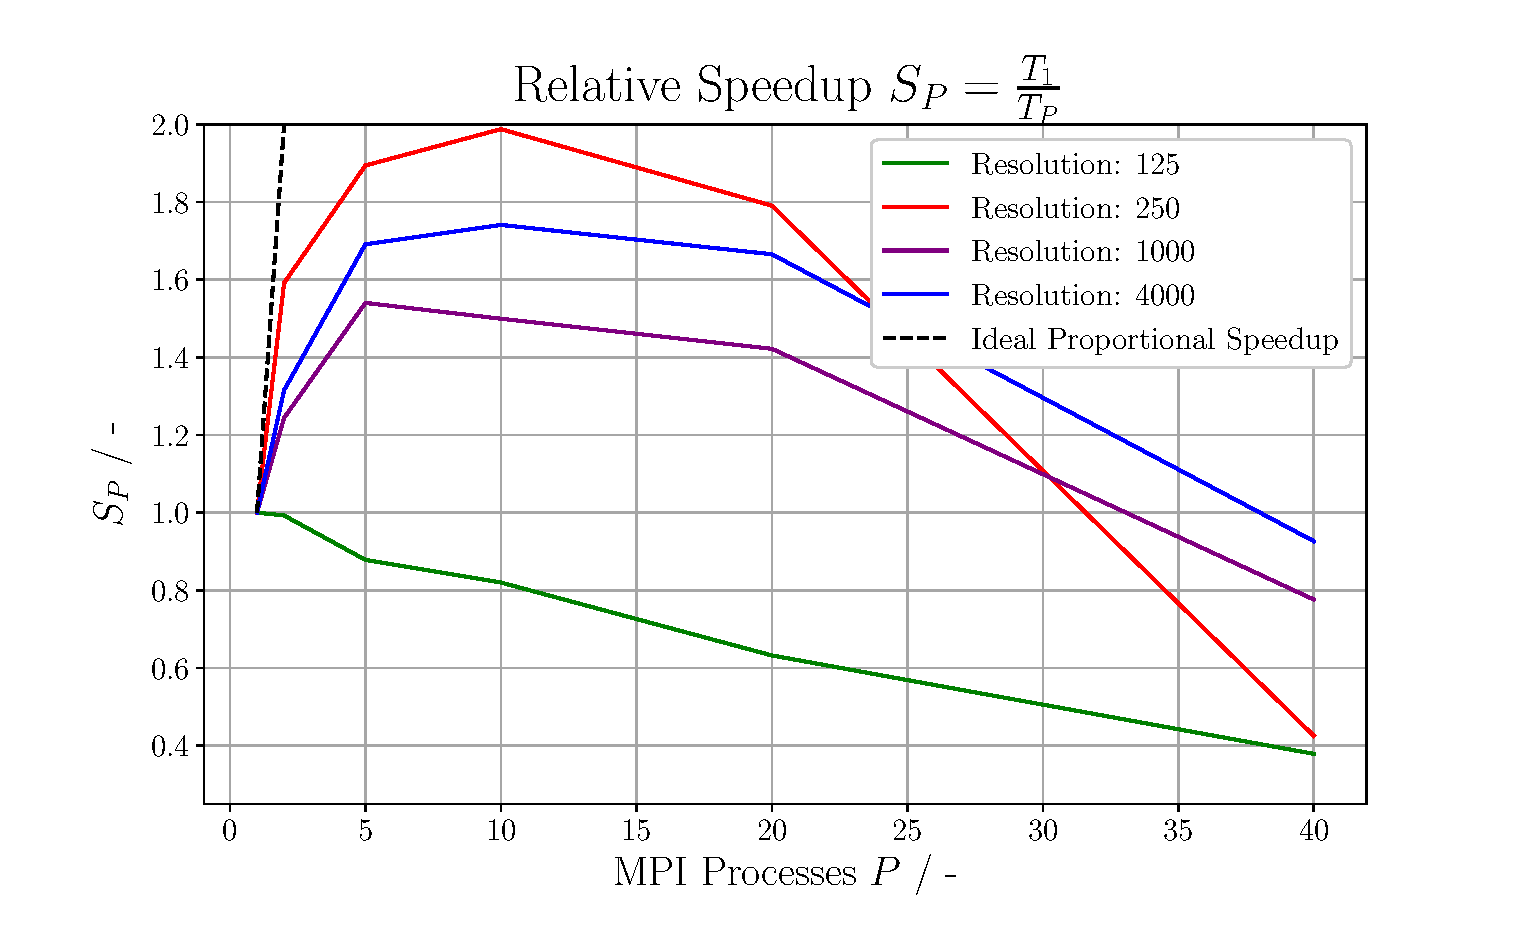
\includegraphics[width=1\textwidth]{figures/S_P_rel.eps}
	\caption{Parallel Speedup for 1D Decomposition of $\Omega$ with 1, 2, 5, 10, 20 and 40 Processes}
	\label{speedup_fig}
\end{figure}

For a grid resolution of 125, one can identify the dominance of the parallelization overhead in figure \ref*{speedup_fig} since it drops below 1 for 2 processes already.
The best speedup out of the 4 discretizations, was achieved by the 250 grid resolution (red graph in \ref*{speedup_fig}).
For 2 processes, said grid resolution lead to almost linear proportional speedup. Its maximum speedup for the chosen processes can be observed
at 10 processes with a speedup factor of almost 2. For 40 processes, one can observe the expected behaviour, where larger problems benefit from parallelization
and the largest problem has the highest speedup and the smallest problem the smallest speedup, which can also be observed in figure \ref*{efficiency_fig},
which is obvious since both figures stem from the same data.

\pagebreak

\begin{figure}[ht]
	\centering
    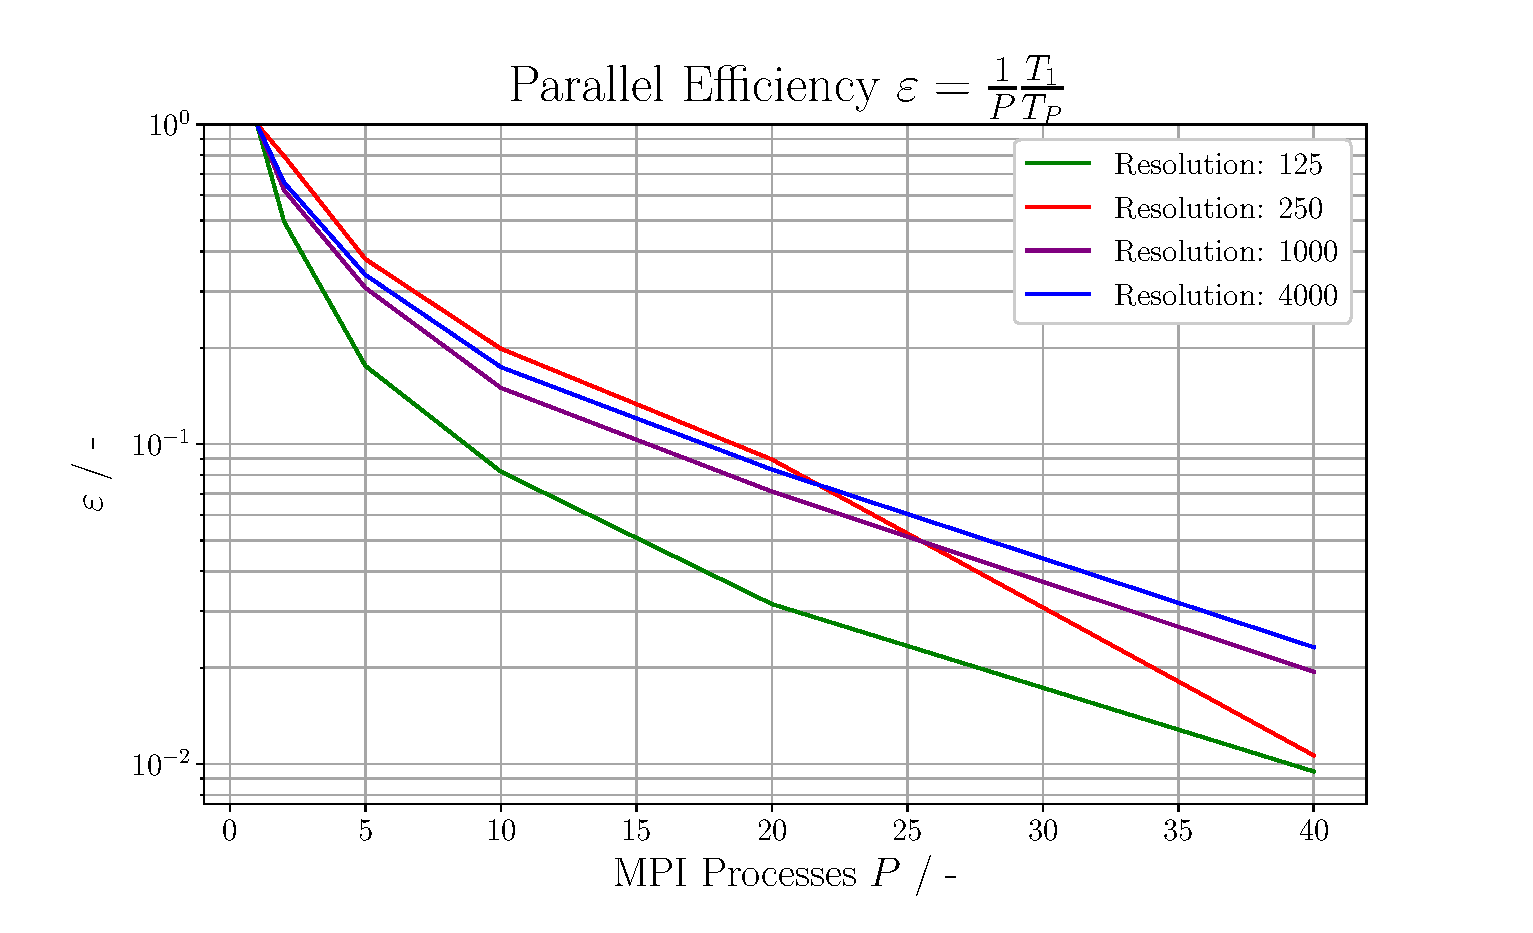
\includegraphics[width=1\textwidth]{figures/epsilon_semilogy.eps}
	\caption{Parallel Efficiency for 1D Decomposition of $\Omega$ with 1, 2, 5, 10, 20 and 40 Processes}
    \label{efficiency_fig}
\end{figure}

In figure \ref*{efficiency_fig} above, the parallel efficiency is shown over \texttt{MPI}-processes.
Visible is again the overhead dominance in the low grid resolution of 125, leading to the overall lowest parallel efficiency for the compared cases.
This overhead dominance leads to a significant efficiency drop for a grid resolution of 250 as well, but only for the jump from 20 to 40 \texttt{MPI} processes.
Again since speedup and efficiency stem from the same data, the large problem size of grid resolution 4000 benefits from parallelization and
has therefore the best parallel efficieny out of the 4 cases.





\pagebreak

%%%%%%%%%%%%%%%%%%%%%%%%%%%%%%%%%%%%%%%%%%%%%%%%%%%%%%%%%%%
%%%%%%%%%%%%%%%%%%%%%%%%%%%%%%%%%%%%%%%%%%%%%%%%%%%%%%%%%%%
%%%%%%%%%%%%%%%%%%%%%%%%%%%%%%%%%%%%%%%%%%%%%%%%%%%%%%%%%%%
%%%%%%%%%%%%%%%%%%%%%%%%%%%%%%%%%%%%%%%%%%%%%%%%%%%%%%%%%

%% During the document writing process, this single .tex file is used to let you write down a little to do list, just comment it out when the paper is done!
%\section{To Do's}





- What's still to you do make your supervisor/prof happy?

\begin{figure}[ht]
	\centering
  
\includegraphics[width=0.7\textwidth]{figures/bild_1}
	\caption{gestaucht}
	\label{lbl_bild_1}
\end{figure}




\pagebreak






%%%%%%%%%%%%%%%%%%%%%%%%%%%%%%%%%%%%%%%%%%%%%%%%%%%%%%%%%%%
%%%%%%%%%%%%%%%%%%%%%%%%%%%%%%%%%%%%%%%%%%%%%%%%%%%%%%%%%%%
%%%%%%%%%%%%%%%%%%%%%%%%%%%%%%%%%%%%%%%%%%%%%%%%%%%%%%%%%%%
%%%%%%%%%%%%%%%%%%%%%%%%%%%%%%%%%%%%%%%%%%%%%%%%%%%%%%%%%

%%% Bibliography printing at this point! 
%\printbibliography

%%% This is a hardcoded string to enforce it in the table of contents, if you want your "references" string in the TOC to be named differently, such as bibliography or so on, just change the third input to this command below to your desired references naming that should appear in the TOC
%\addcontentsline{toc}{section}{References}


%\pagebreak

%%%%%%%%%%%%%%%%%%%%%%%%%%%%%%%%%%%%%%%%%%%%%%%%%%%%%%%%%%%
%%%%%%%%%%%%%%%%%%%%%%%%%%%%%%%%%%%%%%%%%%%%%%%%%%%%%%%%%%%
%%%%%%%%%%%%%%%%%%%%%%%%%%%%%%%%%%%%%%%%%%%%%%%%%%%%%%%%%%%


%%% This is where the appendix .tex file is included, the settings to the appendix are changed in the settings.tex file
%\begin{appendix}
\addappheadtotoc
\section{Python Code Listing}
\label{app_a}

Here is an example of a python listing, you can change appearance of comments, strings, numbering, known commands and variables in the package settings in packages.tex. You can obviously use the listings environment in the rest of the document. The same procedure applies for listings in other languages.


\vfill

\begin{lstlisting}[language=Python, title=Python Listing Title]
# Python Script, API Version = V18

import math

#    DELETE EVERYTHING  -----------------------------

ClearAll()

#    PARAMETERS  --------------------------------------

w = float(Parameters.w)      # side length of one element or half of a unit cell
e = float(Parameters.e)      # rectangle ratio e
b = w/(1+e)               
rho = float(Parameters.rho)  # relative density
f = float(Parameters.f)      # number of layers = folds+1
h = 2*w/f          # layer height = size of a unit cell divided by the number of layers
f = int(Parameters.f)

# Calculation of wall thickness t
t1 = ((math.sqrt(1-rho)+1)*math.sqrt(2)*w)/2
t2 = -((math.sqrt(1-rho)-1)*math.sqrt(2)*w)/2
if t1 <t2:
  t=t1
else:
   t=t2
   
# auxiliary variable to build up rectangle
m = math.sqrt(pow(t,2)*2)/2

\end{lstlisting}


\vfill

\pagebreak


\section{XMl Code Listing}
Here is an example for XML code listing.
\vfill

\begin{lstlisting}[language=XML, title=XML Listing Title]
<extension version="1" name="EnergyIntegral" loadasdefault="True">
  <guid shortid="EnergyIntegral">8005c624-8869-4c74-b32b-97ac59c200b2</guid>                                  
  <script src="energy_integral.py" />
  <interface context="Mechanical">
\end{lstlisting}

\vfill


\pagebreak


\section{MATLAB Code Listing}
Here is an example for MATLAB code listing

\vfill

\begin{lstlisting}[language=MATLAB,title=MATLAB Listing Title]
%% Linear model Poly44 from MATLAB Curve Fit App:

%Polynomial Coefficients (with 95\% confidence bounds):
       p00 =       13.79;  %(13.22, 14.36)
       p10 =      -2.897;  %(-3.454, -2.34)
       p01 =       3.752;  %(3.163, 4.34)
       p20 =       3.279;  %(2.231, 4.327)
       p11 =      0.5404;  %(-0.2001, 1.281)
       p02 =      0.8638;  %(-0.4624, 2.19)
       p30 =       0.299;  %(0.01281, 0.5851)
       p21 =     -0.5091;  %(-0.7299, -0.2884)
       p12 =      0.4973;  %(0.2716, 0.7229)
       p03 =      0.3595;  %(0.04484, 0.6741)
       p40 =     -0.8495;  %(-1.291, -0.4084)
       p31 =    -0.02258;  %(-0.3136, 0.2685)
       p22 =     -0.2819;  %(-0.5502, -0.01351)
       p13 =      0.2674;  %(-0.05265, 0.5874)
       p04 =      0.2019;  %(-0.3968, 0.8006)
       
  	f(x,y) = p00 + p10*x + p01*y + p20*x^2 + p11*x*y + p02*y^2 + p30*x^3 + p21*x^2*y 
  	+ p12*x*y^2 + p03*y^3 + p40*x^4 + p31*x^3*y + p22*x^2*y^2 
  	+ p13*x*y^3 + p04*y^4

  %Goodness of fit:
  %SSE: 3.189
  %R-square: 0.9949
  %Adjusted R-square: 0.9902
  %RMSE: 0.4611
\end{lstlisting}

\vfill

\end{appendix}


%%%%%%%%%%%%%%%%%%%%%%%%%%%%%%%%%%%%%%%%%%%%%%%%%%%%%%%%%%%
%%%%%%%%%%%%%%%%%%%%%%%%%%%%%%%%%%%%%%%%%%%%%%%%%%%%%%%%%%%
%%%%%%%%%%%%%%%%%%%%%%%%%%%%%%%%%%%%%%%%%%%%%%%%%%%%%%%%%%%


\end{document}

